\documentclass[9pt,twocolumn]{article}
\usepackage[margin=0.55in, top=0.62in, bottom=0.58in]{geometry}
\usepackage{amsmath,amssymb,booktabs,graphicx,microtype,url}
\setlength{\columnsep}{0.22in}
\setlength{\parindent}{1em}\setlength{\parskip}{1pt}
\title{Munchkin: Reinforcement Learning for Dynamic Food-Delivery Dispatch}
\author{Anshit Agarwal \and Namya Dhingra\\\small GitHub: \url{https://github.com/Anshit2005/Munchkin---RL-Based-Dynamic-Food-Delivery-Dispatch-System}}
\date{}
\begin{document}\maketitle\begin{abstract}
We present Munchkin, a minute-stepped food-delivery dispatch simulator and comparative study of three dispatch heuristics, Deep Q-Network (DQN), and Proximal Policy Optimization (PPO). A fixed 60-minute episode couples stochastic order arrivals, restaurant preparation, travel, deadlines, and finite driver capacity. The observation contains 1,849 features and the masked discrete action space contains 1,025 actions. Across 11 five-seed scenario configurations, the heuristics remain highly competitive; learned policies show useful behavior under some constrained conditions but do not dominate consistently.\end{abstract}
\section{Problem and environment}
Munchkin models online assignment of arriving food orders to delivery partners. Each episode simulates one hour: one real-time second corresponds to one game minute. The map is $100\times70$ units, with 3--8 restaurants and 3--16 drivers in training. New orders arrive according to a Poisson process with scenario rate $\lambda\in[1,8]$ orders/minute; half the configured rate is seeded as initial backlog. Preparation time is sampled from a clipped normal distribution (mean 0.5, SD 0.17 min, bounds 0.15--1.0); estimates are log-normal noisy ($\sigma=0.2$). Deadlines equal estimated preparation plus nominal travel time and five minutes of slack. Traffic has light/normal/heavy multipliers 1.2/1.0/0.7, with minute-to-minute noise. Drivers move, prepare, and deliver as simulated time advances; unfinished orders incur a terminal penalty.
\section{RL formulation}
\textbf{State.} At each minute the fixed-size observation $s_t\in\mathbb{R}^{1849}$ concatenates 16 driver records ($11$ values each), 64 order records ($10$ each), a $16\times64$ driver--order ETA matrix, and 9 global features: $16(11)+64(10)+16(64)+9=1849$. Driver features encode presence, position, availability/travel state, destination, remaining distance/time, and food-wait status. Order features encode presence, restaurant/customer coordinates, age, preparation remaining, restaurant load, route length, and deadline slack. Global features include normalized time/horizon, dispatchable/pending/available counts, demand rate, restaurant count, overflow indicator, and traffic ratio. Padding fixes dimensions; masks exclude absent/infeasible pairs.
\textbf{Actions.} The discrete action is either dispatch driver $i$ to order $j$, encoded $64i+j$ for $i<16,j<64$, or WAIT (index 1024), so $|A|=1,025$. Only feasible driver--order pairs are enabled. An assignment consumes no simulated minute, allowing several dispatches before WAIT advances the environment.
\textbf{Reward.} The shared shaped reward per step is
\begin{equation*}r_t=10D_t-2W_t-4L_t-0.1M_t-I_t-5F_t\mathbf{1}[t=T],\end{equation*}
where $D_t$ is newly completed deliveries, $W_t$ pending orders after movement, $L_t$ overdue pending orders, $M_t$ distance moved, $I_t=\min(\text{available drivers},\text{dispatchable unassigned orders})$ (idle-capacity cost), and $F_t$ unfinished pending orders at the 60-minute cutoff. The game score is separately $10$ points per delivery; reported points are not the shaped RL return.
\section{Policies and training}
We compare Nearest Driver, Oldest/Most Urgent (least deadline slack), and Minimum Estimated Delivery Time with DQN and PPO. Both RL agents use action masking and the same observation and reward. DQN uses a pairwise value network, uniform replay (capacity 20,000; batch 128), masked Double-DQN targets, $\gamma=0.99$, learning rate $3\times10^{-4}$, warm-up 32 transitions, updates every four steps, target sync every 1,000 steps, and $\epsilon$ decay 1.0 to 0.05. PPO uses masked categorical actions, clipped objective ($\epsilon=0.2$), $\gamma=0.99$, GAE $\lambda=0.95$, 8 update epochs, minibatches of 128, and learning rate $3\times10^{-4}$. Training samples PPO actions; evaluation uses deterministic masked argmax. Both were trained for 500 episodes with randomized demand, fleet, restaurant count and traffic. Best checkpoints: DQN episode 175 (validation shaped return $-3949.3$) and PPO episode 300 ($-4806.9$). Reported sweep results use five matched seeds per cell, 60-minute episodes (11 configurations, 275 policy-episodes total).
\begin{figure*}[t]\centering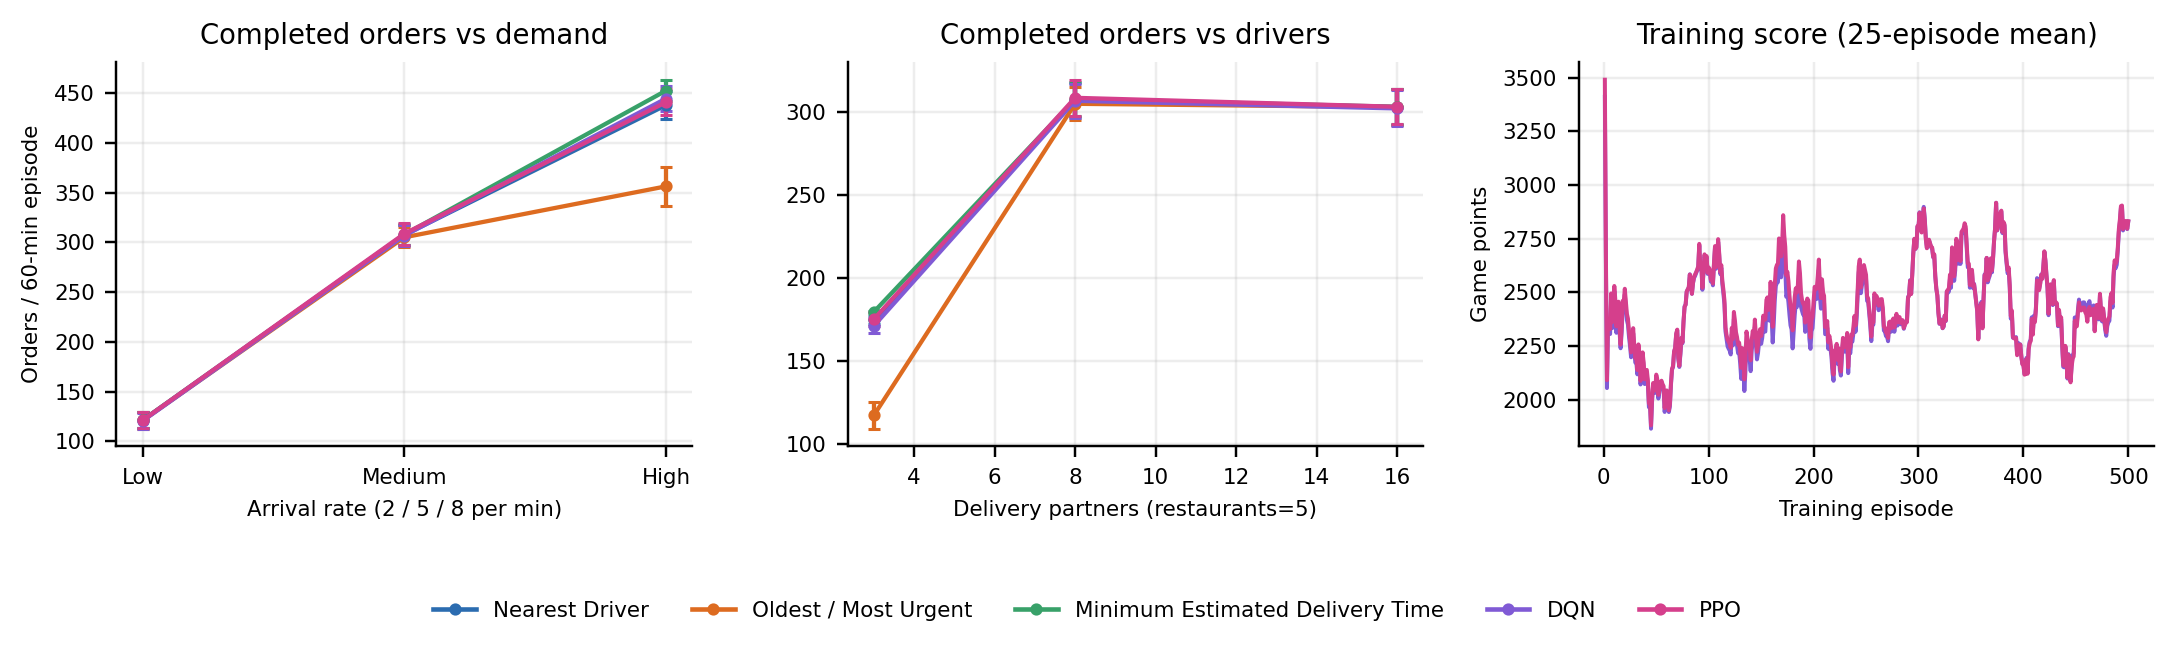
\includegraphics[width=0.97\textwidth]{images/results.png}\caption{Evaluation across demand, driver capacity, and training. Error bars show across-seed SD for completed orders; training curve is a 25-episode moving mean of game points.}\end{figure*}
\section{Results and discussion}
Table~\ref{tab:main} reports deliveries and game points for fixed normal-traffic scenarios (five seeds each). At low and medium demand, methods are close; PPO leads medium-demand points (3,086), while Minimum ETA is similar (3,078). At high demand, Minimum ETA delivers most (452.4); DQN is lower (444.4) but has the best mean shaped return among the five policies (−1,184 versus −1,681 for Minimum ETA). Hence the shaped reward and game score rank policies differently. In the medium-demand, three-driver case, Minimum ETA completes 179.4 orders versus DQN 171.0 and PPO 175.0. In the severe high-demand/heavy-traffic, three-driver stress case, Minimum ETA completes 177.6, PPO 144.6 and DQN 100.4. These results do not support a claim that RL universally outperforms the heuristics; the severe-capacity case exposes a weakness of the learned dispatchers.
\begin{table}[h]\centering\small\caption{Mean completed orders / game points by demand (normal traffic).}\label{tab:main}\begin{tabular}{lrrr}\toprule Policy & Low & Medium & High\\\midrule Nearest &121.2/1212&307.4/3074&437.8/4378\\Urgent &121.0/1210&305.0/3050&356.2/3562\\Min ETA &121.2/1212&307.8/3078&452.4/4524\\DQN &120.6/1206&306.8/3068&444.4/4444\\PPO &121.2/1212&308.6/3086&440.8/4408\\\bottomrule\end{tabular}\end{table}
\textbf{Conclusion.} Munchkin provides a reproducible benchmark with explicit state/action masks and shared scenario dynamics. The current learned policies are competitive in selected regimes but not uniformly superior. Future work should target constrained-fleet credit assignment, broader hyperparameter/reward sweeps, and more seeds before drawing statistical conclusions.\vspace{-2mm}
\begin{thebibliography}{3}\scriptsize\setlength{\itemsep}{-2pt}
\bibitem{dqn} V. Mnih et al., ``Human-level control through deep reinforcement learning,'' \emph{Nature}, 518, 529--533, 2015. doi:10.1038/nature14236.
\bibitem{ppo} J. Schulman et al., ``Proximal Policy Optimization Algorithms,'' arXiv:1707.06347, 2017.
\bibitem{repo} Munchkin project repository and simulator implementation, GitHub, 2026.\end{thebibliography}
\end{document}
